\chapter{Point Reactor Kinetics}
\label{ch:pk}

The point reactor kinetics (PRK) equations are the dynamical backbone of this
book. They describe how reactor power evolves in time under a prescribed
reactivity, and they make explicit the decisive role of delayed neutrons. We
derive them, solve them in the cases that matter for stability, and extract the
two results---the inhour equation and the prompt-jump approximation---that we
will use again and again.

\section{Delayed neutrons}

Most fission neutrons are emitted within $10^{-14}\unit{s}$ of fission: these are
\emph{prompt}. A small fraction, however, appear with a delay, emitted by certain
neutron-rich fission products (``precursors'') as they beta-decay. The classic
example is $^{87}$Br, which decays to an excited $^{87}$Kr that promptly emits a
neutron; the effective delay is set by the $55\unit{s}$ half-life of the bromine.
In practice the many precursors are grouped into six (sometimes eight) effective
groups, each with a yield fraction $\beta_i$ and a decay constant $\lambda_i$.

The total delayed fraction is
\begin{equation}
\beta = \sum_{i=1}^{6}\beta_i \approx 0.0065 \ \text{for }^{235}\text{U (thermal)},
\end{equation}
with group decay constants ranging from $\lambda_1\approx0.0124\unit{s^{-1}}$
(half-life $\sim 56\unit{s}$) to $\lambda_6\approx 3.0\!-\!3.9\unit{s^{-1}}$
(half-life under a second). Although less than one neutron in a hundred is
delayed, these neutrons set the timescale of the controllable reactor: their
mean delay, of order $10\unit{s}$, vastly exceeds the prompt generation time
$\Lambda\sim 10^{-5}\unit{s}$, so the \emph{average} neutron lifetime weighted by
prompt and delayed contributions is dominated by the delayed term whenever the
reactor is below prompt criticality. Appendix~A lists the full data set.

\section{Derivation of the PRK equations}

Let $n(t)$ be the neutron population (proportional to power $P$) and $C_i(t)$ the
concentration of precursor group $i$. In one generation, $\keff$ neutrons are
produced per neutron; of these, a fraction $(1-\beta)$ are prompt and a fraction
$\beta_i$ feed precursor group $i$. The prompt balance gives a production rate
$(1-\beta)\keff n/\ell$ against a loss rate $n/\ell$, while each precursor group
gains at rate $\beta_i \keff n/\ell$ and loses by decay at rate $\lambda_i C_i$;
the decay of precursors returns neutrons at rate $\lambda_i C_i$. Writing
$\Lambda=\ell/\keff$ and using $\rho=(\keff-1)/\keff$, the result is the standard
six-group point reactor kinetics equations:
\begin{equation}
\boxed{\;
\begin{aligned}
\frac{\dd n}{\dd t}
  &= \frac{\rho(t)-\beta}{\Lambda}\, n(t) + \sum_{i=1}^{6}\lambda_i C_i(t),\\[4pt]
\frac{\dd C_i}{\dd t}
  &= \frac{\beta_i}{\Lambda}\, n(t) - \lambda_i C_i(t),
  \qquad i=1,\dots,6.
\end{aligned}\;}
\label{eq:prk}
\end{equation}
The same equations hold with $n$ replaced by power $P$, since the two are
proportional in the point approximation. In normalised form we write $p=P/P_0$.

The structure of \eqref{eq:prk} is already revealing. The prompt coefficient
$(\rho-\beta)/\Lambda$ changes sign at $\rho=\beta$. Below it, the coefficient is
\emph{negative}: the prompt chain alone would die away, and the population is held
up only by the slow return of delayed neutrons through $\sum\lambda_iC_i$. This
is the regime of controllable operation. Above it, $\rho>\beta$, the prompt
coefficient is positive and the population grows on the $\Lambda$ timescale
regardless of the delayed neutrons---prompt criticality.

\section{Steady state and the initial condition}

At constant power $p_0$ with $\rho=0$, the time derivatives vanish and
\begin{equation}
C_{i,0} = \frac{\beta_i}{\lambda_i\Lambda}\, p_0,
\label{eq:prk-ss}
\end{equation}
which is the equilibrium precursor inventory. The precursors hold a large reservoir
of ``stored'' delayed neutrons: because $\lambda_i\Lambda\ll\beta_i$, the
equilibrium $C_{i,0}$ greatly exceeds $p_0$. This reservoir is what gives the
reactor its inertia and is the physical reason the prompt-jump (below) is finite.

\section{The prompt jump approximation}

Consider a step insertion of reactivity $\rho<\beta$ at $t=0$ on a reactor at
steady power. Immediately after the step, the precursor concentrations cannot
change instantaneously (they evolve on the slow $\lambda_i$ timescale), so the
$\sum\lambda_iC_i$ term is momentarily fixed at its pre-step value. The fast
prompt dynamics then drive $n$ to a new quasi-equilibrium on the $\Lambda$
timescale. Setting $\dd n/\dd t\to 0$ in \eqref{eq:prk} with the precursor term
held fixed yields the \textbf{prompt-jump approximation}:
\begin{equation}
\boxed{\ \frac{n(0^+)}{n(0^-)} = \frac{\beta}{\beta-\rho}\ }
\label{eq:promptjump}
\end{equation}
The power jumps essentially instantly by this factor, then rises (or falls) more
slowly as the precursors readjust. For $\rho=0.5\$$ ($\rho=0.5\beta$) the jump is
a factor of two; as $\rho\to\beta^-$ the predicted jump diverges, signalling the
breakdown of the approximation and the onset of prompt criticality. The
prompt-jump captures the ``instant'' part of a transient and is invaluable for
estimating the immediate consequence of a reactivity insertion.

\section{The inhour equation}

To find the asymptotic behaviour, seek exponential solutions $n,C_i\propto
e^{st}$ for constant $\rho$. Substituting into \eqref{eq:prk} gives
$C_i = \beta_i n/[\Lambda(s+\lambda_i)]$, and \eqref{eq:prk} becomes the
\textbf{inhour equation}:
\begin{equation}
\boxed{\ \rho = \Lambda s + \sum_{i=1}^{6}\frac{\beta_i\, s}{s+\lambda_i}\ }
\label{eq:inhour}
\end{equation}
This transcendental equation has seven real roots $s_j$ for six delayed groups.
The roots interlace the negative poles $-\lambda_i$; six of them are negative
(decaying transients), and one---the \emph{dominant} root---has the sign of
$\rho$. The reactor period is $T=1/s_{\text{dominant}}$, the time for the power to
change by a factor $e$.

For small positive reactivity the dominant root is small, $s\approx
\rho/(\beta-\rho)\cdot \bar\lambda^{-1}$ in a one-group caricature, giving a long
(stable, slow) period dominated by the delayed neutrons. As $\rho\to\beta$ the
dominant root grows rapidly and the period collapses; beyond $\beta$ the leading
behaviour is $s\approx(\rho-\beta)/\Lambda$, the prompt period.

\begin{figure}[H]
\centering
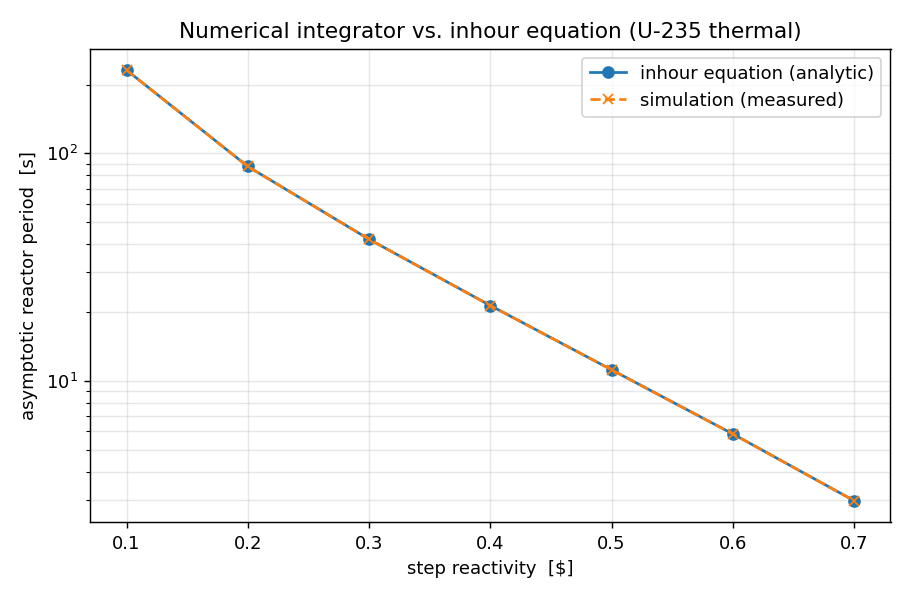
\includegraphics[width=0.74\linewidth]{figures/inhour_validation.png}
\caption{Asymptotic reactor period as a function of step reactivity for
$^{235}$U thermal data. The closed-form inhour solution (solid) and a direct
numerical integration of \eqref{eq:prk} (dashed) agree to
better than $10^{-4}$. Note the steep collapse of the period as reactivity
approaches one dollar.}
\label{fig:inhour}
\end{figure}

\begin{example}[The danger of one dollar]
With $\Lambda=10^{-5}\unit{s}$ and $\beta=0.0065$, a reactivity of
$0.5\$=325\unit{pcm}$ gives a stable period of tens of seconds---easily
controllable. A reactivity of $1.5\$=975\unit{pcm}$ is $0.5\$$ above prompt
critical; the dominant root is approximately
$s\approx(\rho-\beta)/\Lambda=(0.00975-0.0065)/10^{-5}\approx 325\unit{s^{-1}}$,
an e-folding every $3\unit{ms}$. Power rises by a factor of $e^{10}\approx
2\times10^{4}$ in just $30\unit{ms}$. No mechanical system can intervene on that
timescale; only the prompt negative feedback of the fuel (Doppler) can, if it
exists and has the right sign.
\end{example}

\section{Numerical solution and stiffness}

For time-varying $\rho(t)$, or with feedback, \eqref{eq:prk}
must be integrated numerically. The system is \emph{stiff}: it contains the very
fast prompt timescale $\Lambda$ alongside the slow precursor timescales
$1/\lambda_i$, spanning six orders of magnitude. Explicit integrators require
prohibitively small steps; implicit or specialised stiff methods (backward
differentiation, LSODA, or analytic-within-a-step schemes) are standard.
Figure~\ref{fig:transients} shows representative transients computed this way:
a sub-prompt step settling onto a stable period, a prompt-critical excursion
diverging on the millisecond scale, a control-rod scram, and---most
importantly for stability---a reactivity-initiated transient that is turned over
by negative temperature feedback. The last of these is the prototype of a
\emph{thermally stable} response, and the contrast with the un-fed-back
prompt-critical case is the whole subject of the book in one picture.

\begin{figure}[H]
\centering
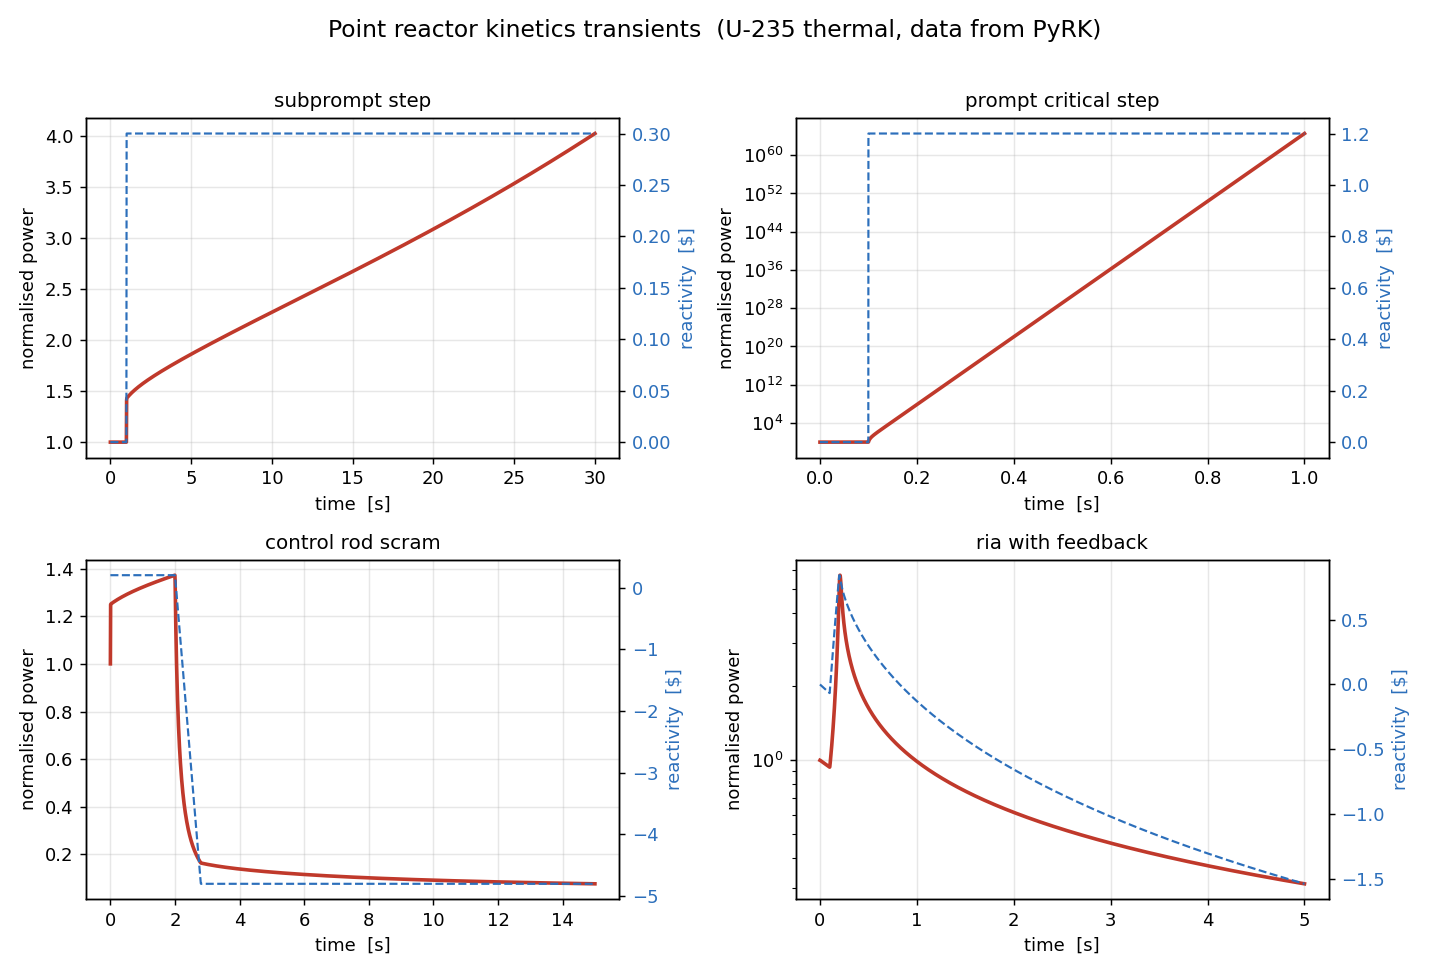
\includegraphics[width=\linewidth]{figures/transients.png}
\caption{Point-kinetics transients for $^{235}$U thermal data. Top left: a
sub-prompt $+0.3\$$ step (stable period). Top right: a prompt-critical $+1.2\$$
step (runaway, log scale). Bottom left: a control-rod scram. Bottom right: a
reactivity-initiated excursion limited by negative feedback---the signature of
thermal stability.}
\label{fig:transients}
\end{figure}

\keypoint{The point kinetics equations contain the entire timescale problem of
reactor control. Below one dollar, delayed neutrons stretch the response to
seconds and the reactor is controllable. Above one dollar, the response collapses
to the prompt timescale and only instantaneous feedback can save the reactor.
Everything that follows---feedback coefficients, stability criteria, the
Chernobyl excursion---is about staying below that line, or about what happens
when a machine crosses it.}



\section{Matrix formulation and spectral theory}
\label{sec:pk-matrix}

Write the state $\mathbf y=(n,C_1,\dots,C_G)^{\!\top}\in\mathbb R^{G+1}$. For
constant $\rho$ the point kinetics \eqref{eq:prk} are the linear system
$\dot{\mathbf y}=\mathbf M(\rho)\mathbf y$ with
\begin{equation}
\mathbf M(\rho)=
\begin{pmatrix}
\dfrac{\rho-\beta}{\Lambda} & \lambda_1 & \cdots & \lambda_G\\[5pt]
\dfrac{\beta_1}{\Lambda} & -\lambda_1 & & \\
\vdots & & \ddots & \\
\dfrac{\beta_G}{\Lambda} & & & -\lambda_G
\end{pmatrix}.
\label{eq:M}
\end{equation}

\begin{theorem}[Spectrum equals inhour roots]
\label{thm:spectrum}
$s\in\sigma(\mathbf M(\rho))$ if and only if $s$ solves the inhour equation
\eqref{eq:inhour}: $\ \rho=\Lambda s+\sum_{i=1}^G \beta_i s/(s+\lambda_i).$
\end{theorem}
\begin{proof}
For an eigenpair $(s,\mathbf y)$ the precursor rows give
$C_i=\frac{\beta_i}{\Lambda(s+\lambda_i)}\,n$ (for $s\ne-\lambda_i$), and the first
row gives $s\,n=\frac{\rho-\beta}{\Lambda}n+\sum_i\lambda_i C_i$. Substituting and
dividing by $n/\Lambda$,
$\Lambda s=\rho-\beta+\sum_i\frac{\lambda_i\beta_i}{s+\lambda_i}$; using
$\lambda_i/(s+\lambda_i)=1-s/(s+\lambda_i)$ yields \eqref{eq:inhour}. The poles
$s=-\lambda_i$ are not eigenvalues (they force $n=0$ and hence $\mathbf y=0$).
\end{proof}

\begin{theorem}[Reality, simplicity, interlacing]
\label{thm:interlacing}
For $\rho\ne0$ the inhour equation has exactly $G+1$ real simple roots
$s_0>s_1>\cdots>s_G$ obeying
$s_0>-\lambda_{(1)}>s_1>-\lambda_{(2)}>\cdots>-\lambda_{(G)}>s_G$, where
$\lambda_{(1)}<\cdots<\lambda_{(G)}$ are the ordered decay constants. Moreover
$\operatorname{sign}(s_0)=\operatorname{sign}(\rho)$.
\end{theorem}
\begin{proof}
Let $h(s)=\Lambda s+\sum_i\beta_i s/(s+\lambda_i)$. Then
$h'(s)=\Lambda+\sum_i\beta_i\lambda_i/(s+\lambda_i)^2>0$ wherever defined, so $h$
is strictly increasing on each interval between consecutive poles, running from
$-\infty$ to $+\infty$ across each; thus $h(s)=\rho$ has exactly one root in each of
the $G$ inter-pole gaps and one to the right of $-\lambda_{(1)}$, giving $G+1$
simple real interlacing roots. Since $h(0)=0$ and $h$ is increasing through the
origin, $\rho>0\Rightarrow s_0>0$ and $\rho<0\Rightarrow s_0<0$.
\end{proof}

\begin{corollary}
The asymptotic period $T=1/s_0$ has the sign of $\rho$, and the solution is
$\mathbf y(t)=\sum_{j=0}^{G}c_j\mathbf v_j e^{s_j t}$ with $\mathbf v_j$ the
eigenvector of $s_j$; for $t\to\infty$ the dominant mode $e^{s_0 t}$ prevails.
\end{corollary}

\begin{proposition}[Nonnegativity of the flow]
\label{prop:metzler}
$\mathbf M(\rho)$ is a Metzler matrix (off-diagonal entries $\ge0$); hence
$e^{\mathbf M t}\ge0$ entrywise for $t\ge0$, and $\mathbf y(0)\ge0$ implies
$\mathbf y(t)\ge0$ for all $t\ge0$. In particular the power $n(t)$ never goes
negative.
\end{proposition}
\begin{proof}
The off-diagonal entries are $\lambda_i\ge0$ and $\beta_i/\Lambda\ge0$; all other
off-diagonal entries vanish. Choose $c>0$ with $\mathbf M+c\mathbf I\ge0$; then
$e^{\mathbf M t}=e^{-ct}e^{(\mathbf M+c\mathbf I)t}$, and the exponential of a
nonnegative matrix is nonnegative (its power series has nonnegative terms). A
nonnegative semigroup maps the nonnegative orthant into itself.
\end{proof}

\paragraph{Prompt jump as a singular perturbation.}
Treat $\Lambda$ as a small parameter. The fast equation
$\Lambda\dot n=(\rho-\beta)n+\Lambda\sum_i\lambda_i C_i$ has, for $\rho<\beta$, a
boundary layer of width $\mathcal O\!\big(\Lambda/(\beta-\rho)\big)$ during which
the slow variables $C_i$ are frozen at their pre-step values. Matching the inner
(layer) solution to the outer quasi-static balance
$n=\Lambda\big(\sum_i\lambda_iC_i\big)/(\beta-\rho)$ gives, at $t=0^+$,
$n(0^+)/n(0^-)=\beta/(\beta-\rho)$, i.e.\ \eqref{eq:promptjump}, with relative error
$\mathcal O(\Lambda)$. This places the prompt-jump approximation on a rigorous
asymptotic footing.


\section*{Exercises}
\addcontentsline{toc}{section}{Exercises}
\begin{enumerate}[leftmargin=*,itemsep=2pt]
\item Derive the steady-state precursor concentration \eqref{eq:prk-ss} from the precursor equation.
\item Compute the prompt-jump factor for $\rho=0.25\$$ and for $\rho=0.9\$$. Comment on the trend as $\rho\to\beta$.
\item Show that the inhour equation \eqref{eq:inhour} has exactly $G+1$ real roots for $G$ delayed groups.
\item For $\rho=1.5\$$, $\Lambda=10^{-5}\,$s, $\beta=0.0065$, estimate the prompt period and the factor by which power grows in $20\,$ms.
\item Explain why the point-kinetics system is numerically stiff and why explicit integrators struggle with it.
\end{enumerate}
